
\documentclass[11pt,a4paper]{article}                           

\usepackage[bookmarksopen, bookmarksnumbered, bookmarksopenlevel=2]{hyperref}
\usepackage{tikz}
\usepackage{tikz-3dplot}
\usetikzlibrary{calc}
\usetikzlibrary{decorations} %
\usepackage{ngerman}
\usepackage[UKenglish]{babel}
\usepackage[toc,page]{appendix}
\usepackage{amsmath}
\usepackage{amssymb}
\usepackage{graphicx}
\usepackage{hhline}
\usepackage[bf]{caption}
\usepackage{cite}
\usepackage[vcentermath]{youngtab}
\usepackage{geometry}
\usepackage{float}
\usepackage{epstopdf}

\usepackage{subfig} % zwei Bilder nebeneinander


\usepackage{wrapfig}	 

\geometry{verbose,a4paper,tmargin=30mm,bmargin=25mm,outer=20mm,inner=20mm,bindingoffset=0mm}
\usepackage{pgfplots}
\pgfplotsset{width=7cm} 

\DeclareSymbolFont{bbold}{U}{bbold}{m}{n}
\DeclareSymbolFontAlphabet{\mathbbold}{bbold}
\newcommand{\one}{\mathbbold{1}}
 



\usepackage{cancel}



%%%%%%%%%%%%%%%%%%%%%%%%%%%%%%%%%%%%%%%%%%%%%%%
%%%%%%%%%%%%%%%%%%%%%%%%%%%%%%%%%%%%%%%%%%%%%%%
%%%%%%%%%%%%%%%%%%%%%%%%%%%%%%%%%%%%%%%%%%%%%%%
%%%%%%%%%%%%%%%%%%%%%%%%%%%%%%%%%%%%%%%%%%%%%%%

%%%%%%%%%%%%%%%%%%%%%%%%%%%%%%%%%%%%%%%%%%%%%%%
\hypersetup{
    pdftitle={},
    pdfauthor={David Gerick},
    pdfsubject={HGSFP Winter School 2017 evaluation}
}
%
%%%%%%%%%%%%%%%%%%%%%%%%%%%%%%%%%%%%%%%%%%%%%%%%%%%%%%%



%%%%%%%%%%%%%%%%%%%%%%%%%%%%%%%%%%%%%%%%%%%%%%%
%%%%%%%%%%%%%%%%%%%%%%%%%%%%%%%%%%%%%%%%%%%%%%%
%%%%%%%%%%%%             %%%%%%%%%%%%%%%%%%%%%%
%%%%%%%%%%%%  TITLEPAGE  %%%%%%%%%%%%%%%%%%%%%%
%%%%%%%%%%%%             %%%%%%%%%%%%%%%%%%%%%%
%%%%%%%%%%%%%%%%%%%%%%%%%%%%%%%%%%%%%%%%%%%%%%%
%%%%%%%%%%%%%%%%%%%%%%%%%%%%%%%%%%%%%%%%%%%%%%%
%%%%%%%%%%%%%%%%%%%%%%%%%%%%%%%%%%%%%%%%%%%%%%%

\begin{document}
\section*{Lecture: N. Berger - "Two, three, many? How quarks make hadrons"}

Dear Niklaus,\\
we would like to thank you so much for being an important part of this year's HGSFP Winter School and for the nice presentation you gave.
In the appendix we present to you the part of the anonymous evaluation which addresses your talk.\\
Also we hope, that you enjoyed the stay in Obergurgl. If you have any questions or remarks, please feel free to contact us via \textbf{winterschool2017@physi.uni-heidelberg.de}. Please also remember to send us your slides to be distributed among the students (the slides will not be made public at any time) and to hand in your travel reimbursement documents, if not already happened.\\
From all of us from the organization team,\\
Heiko, David, Lennart, Frank, Janko and Merve


\begin{figure}[H]
\centering
\null\hfill %
{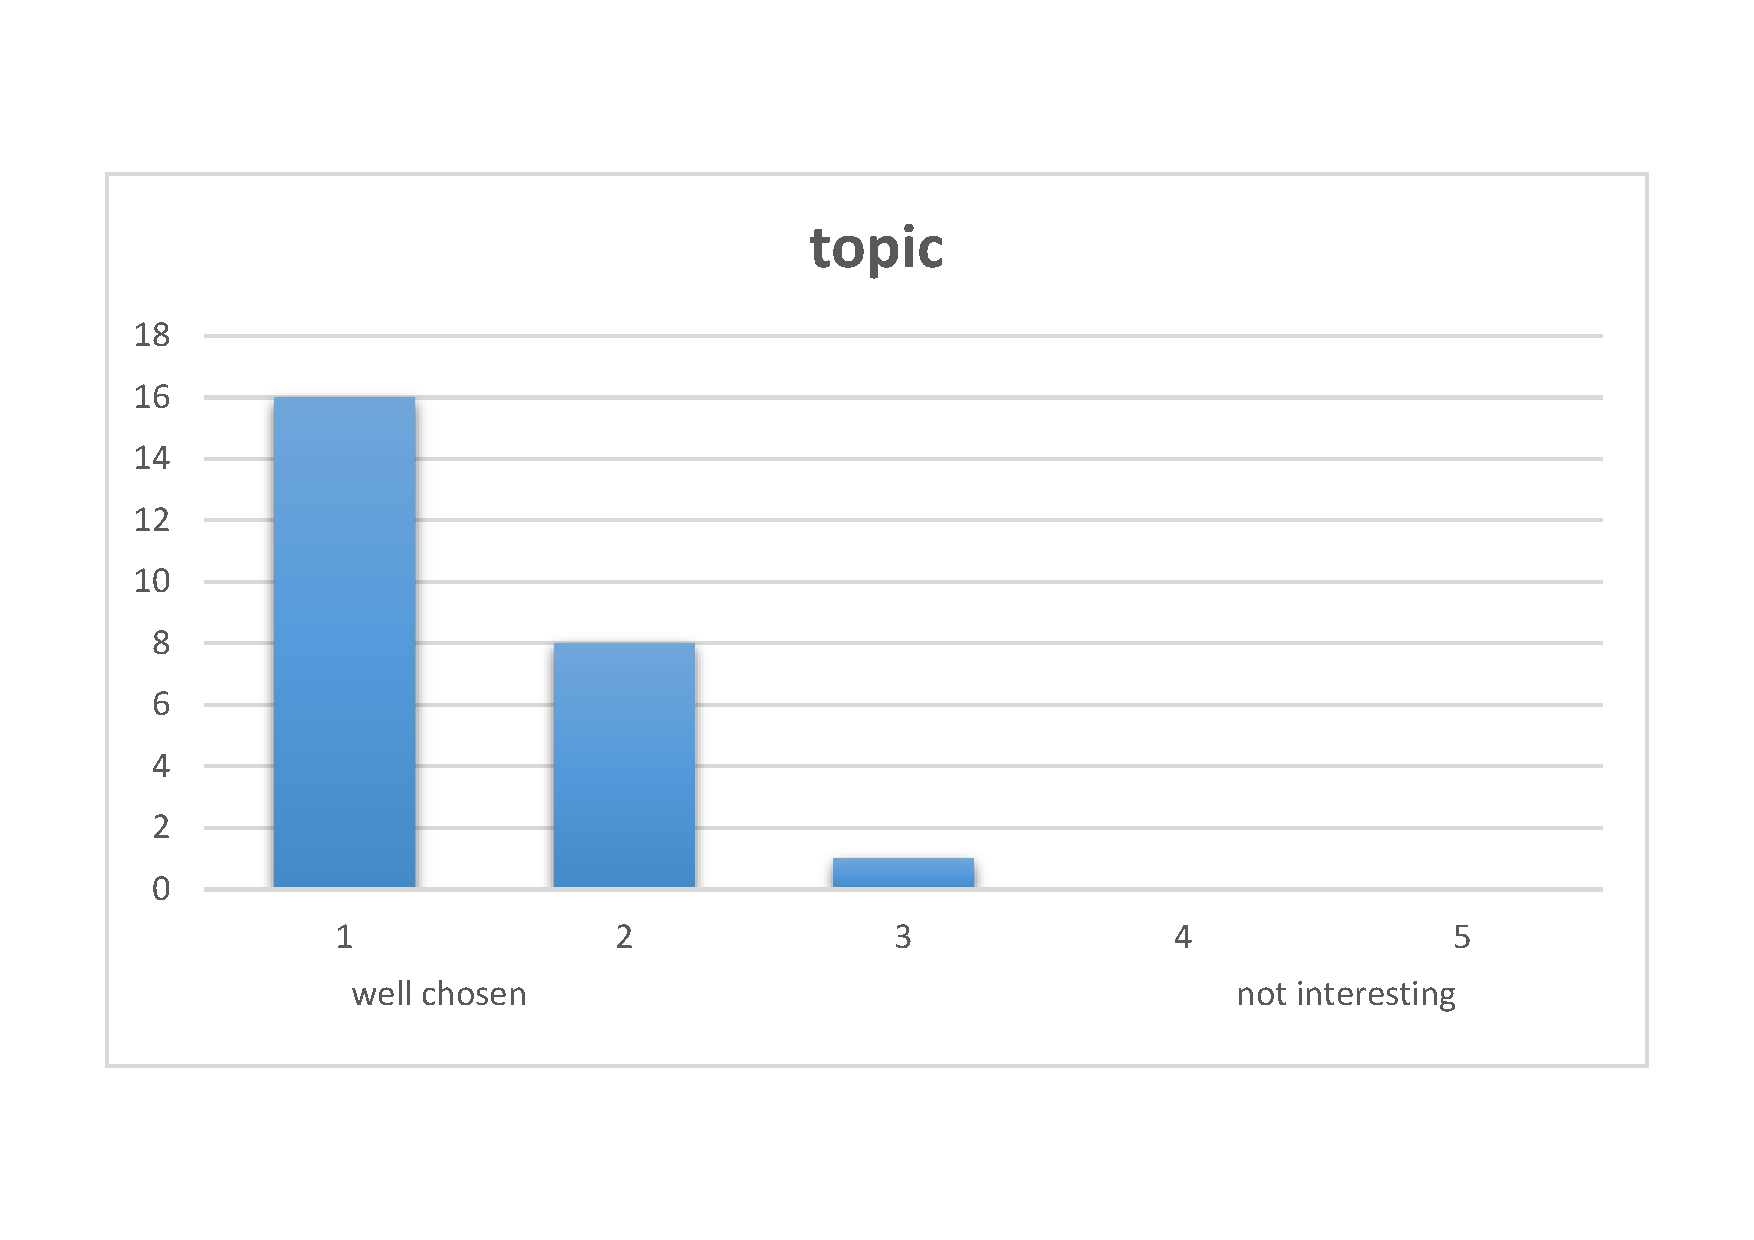
\includegraphics[width=0.49\textwidth]{topic.pdf}}
\hfill %
{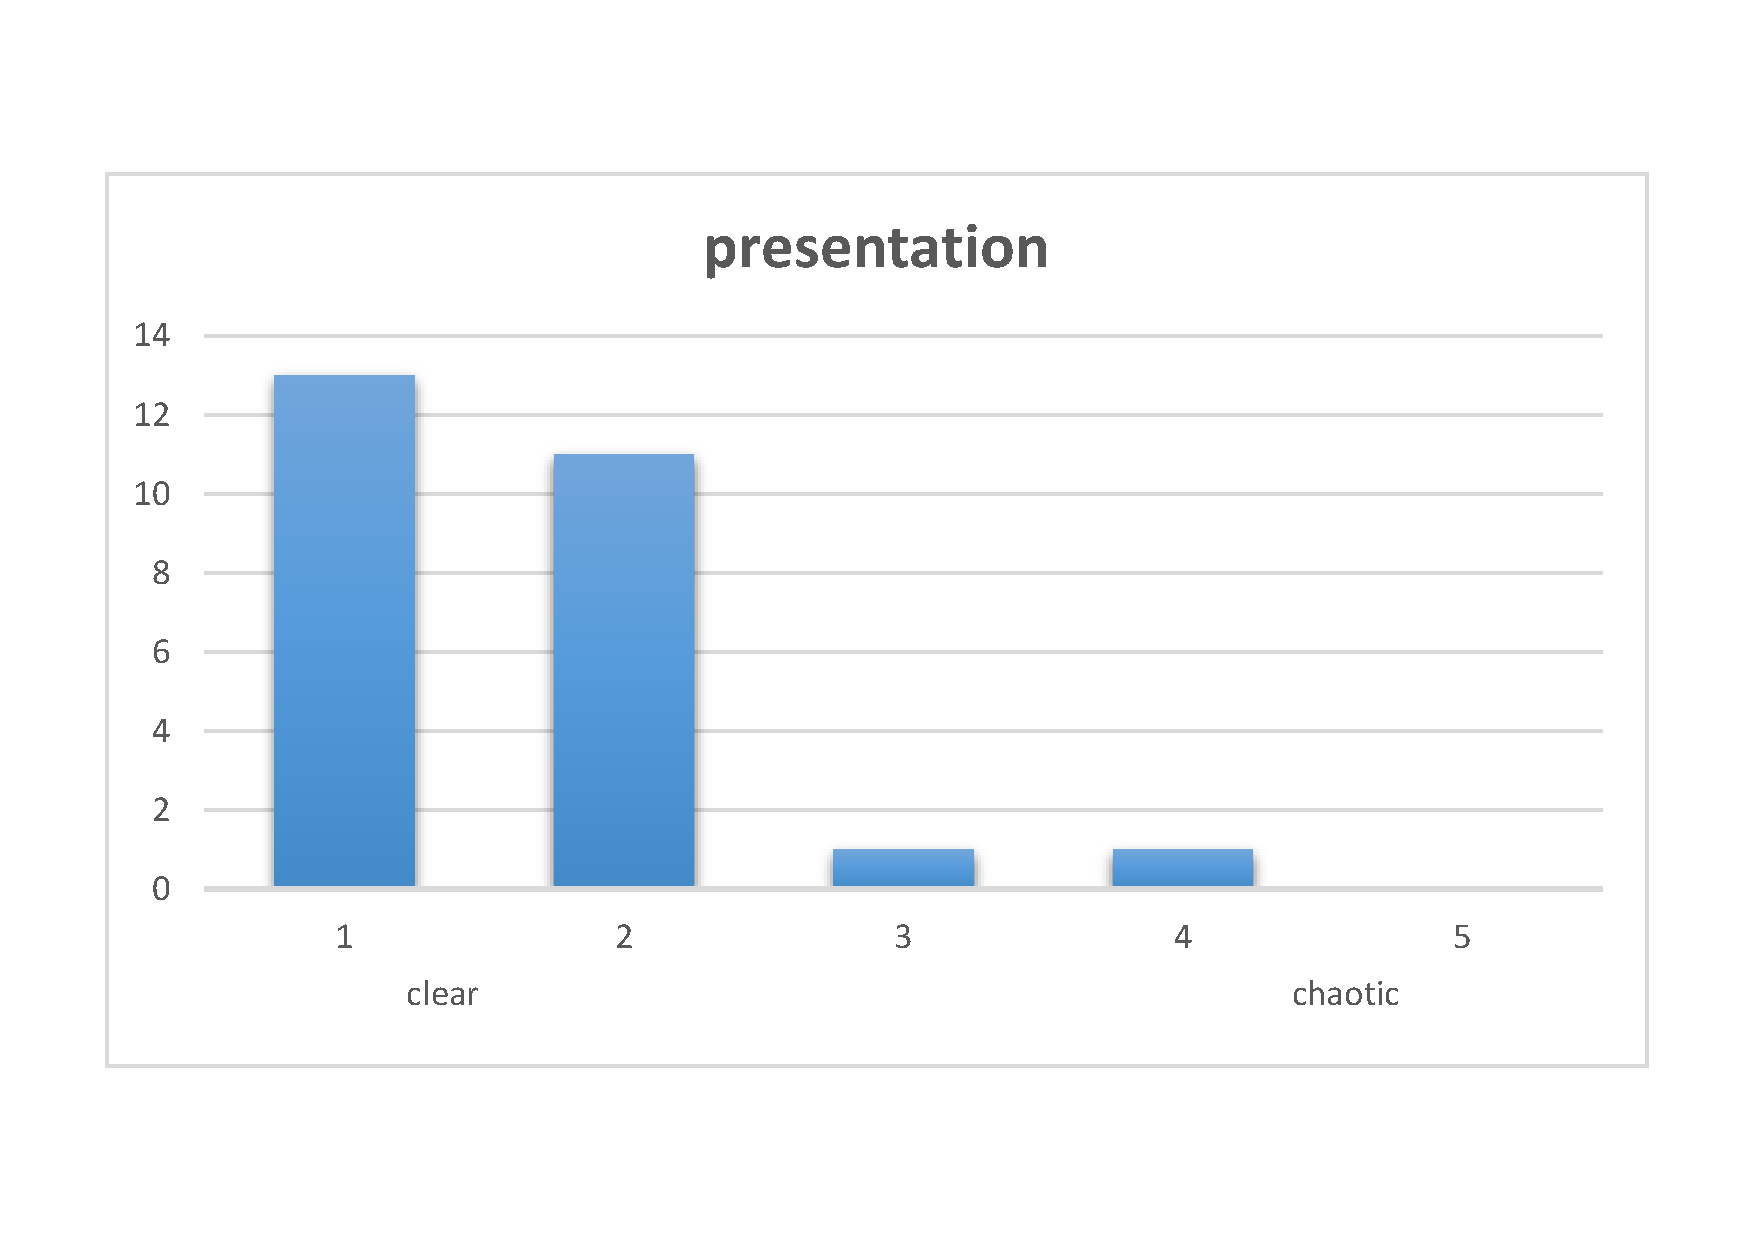
\includegraphics[width=0.49\textwidth]{presentation.pdf}}
\hfill %
{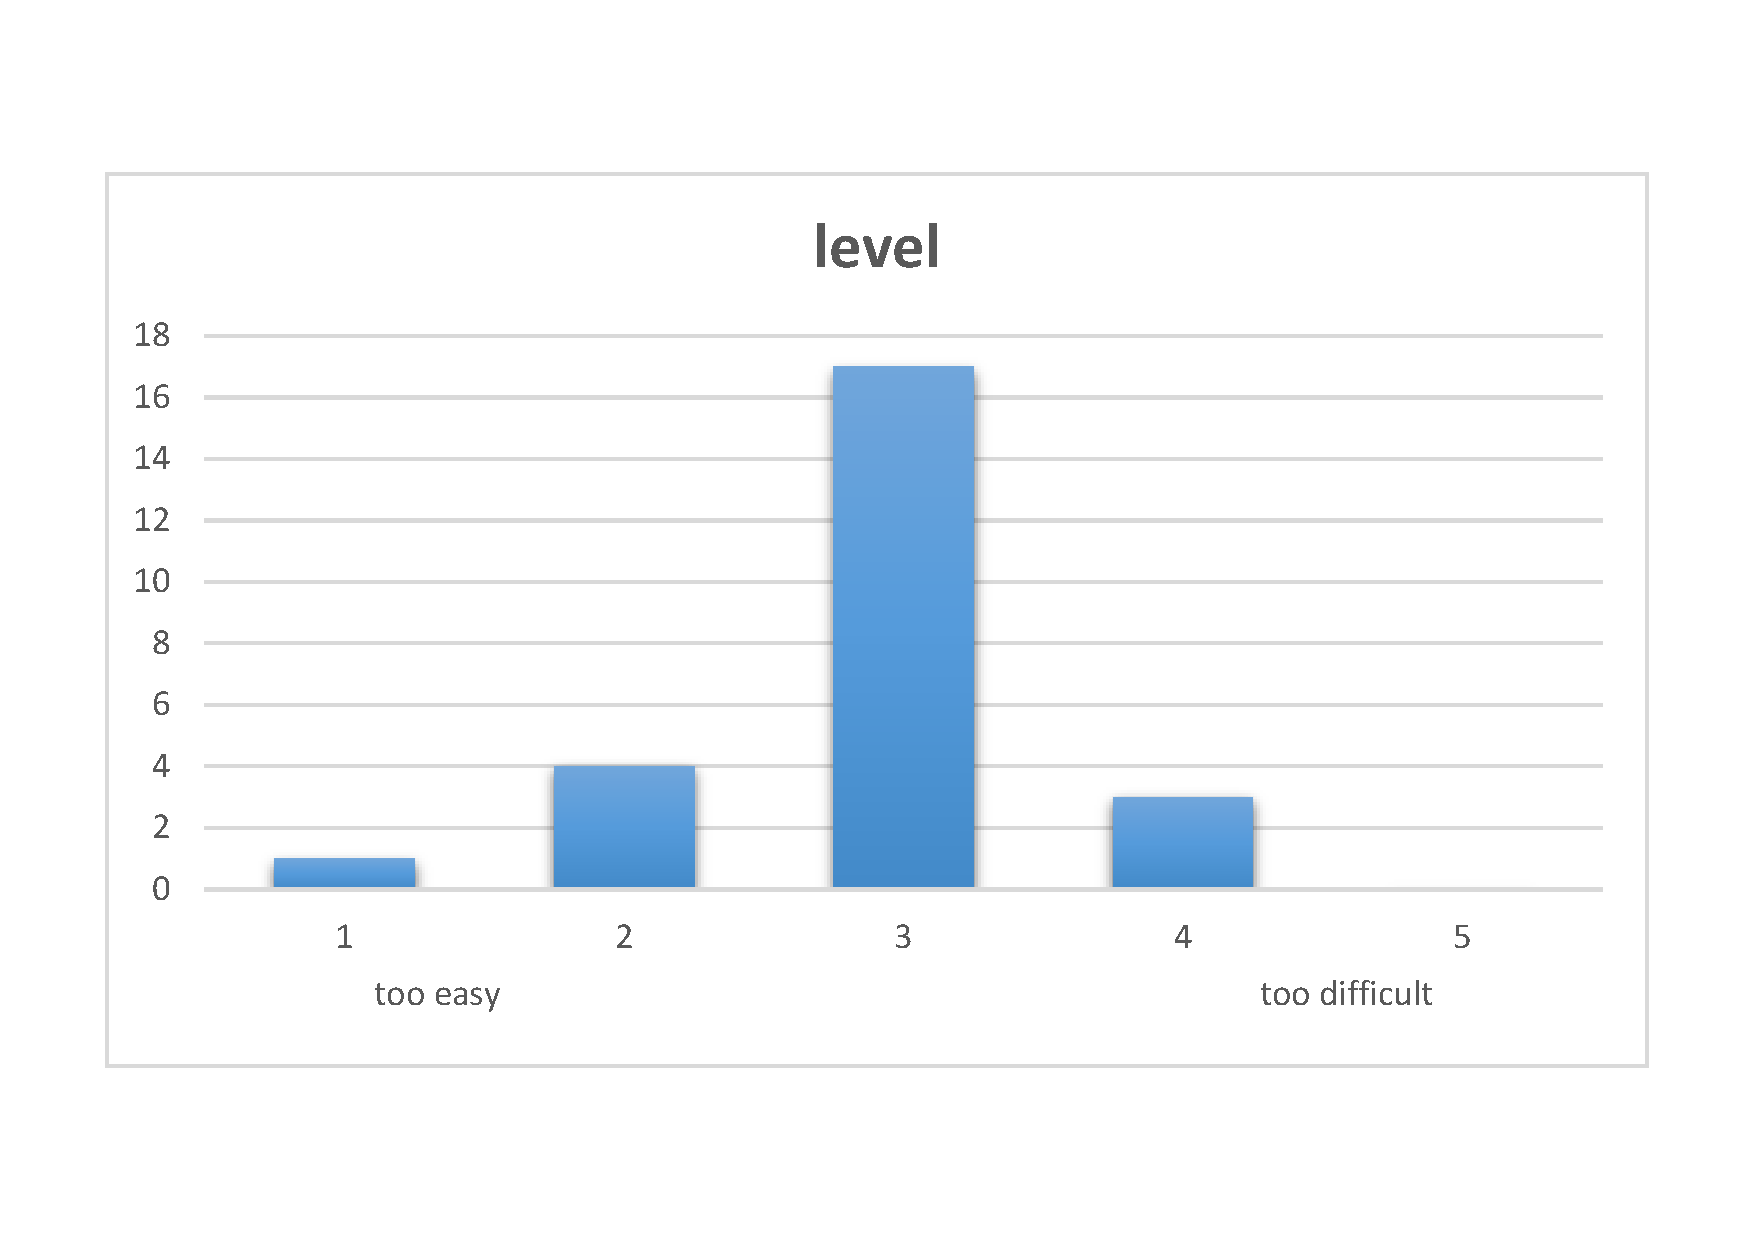
\includegraphics[width=0.49\textwidth]{level.pdf}}
\hfill %
{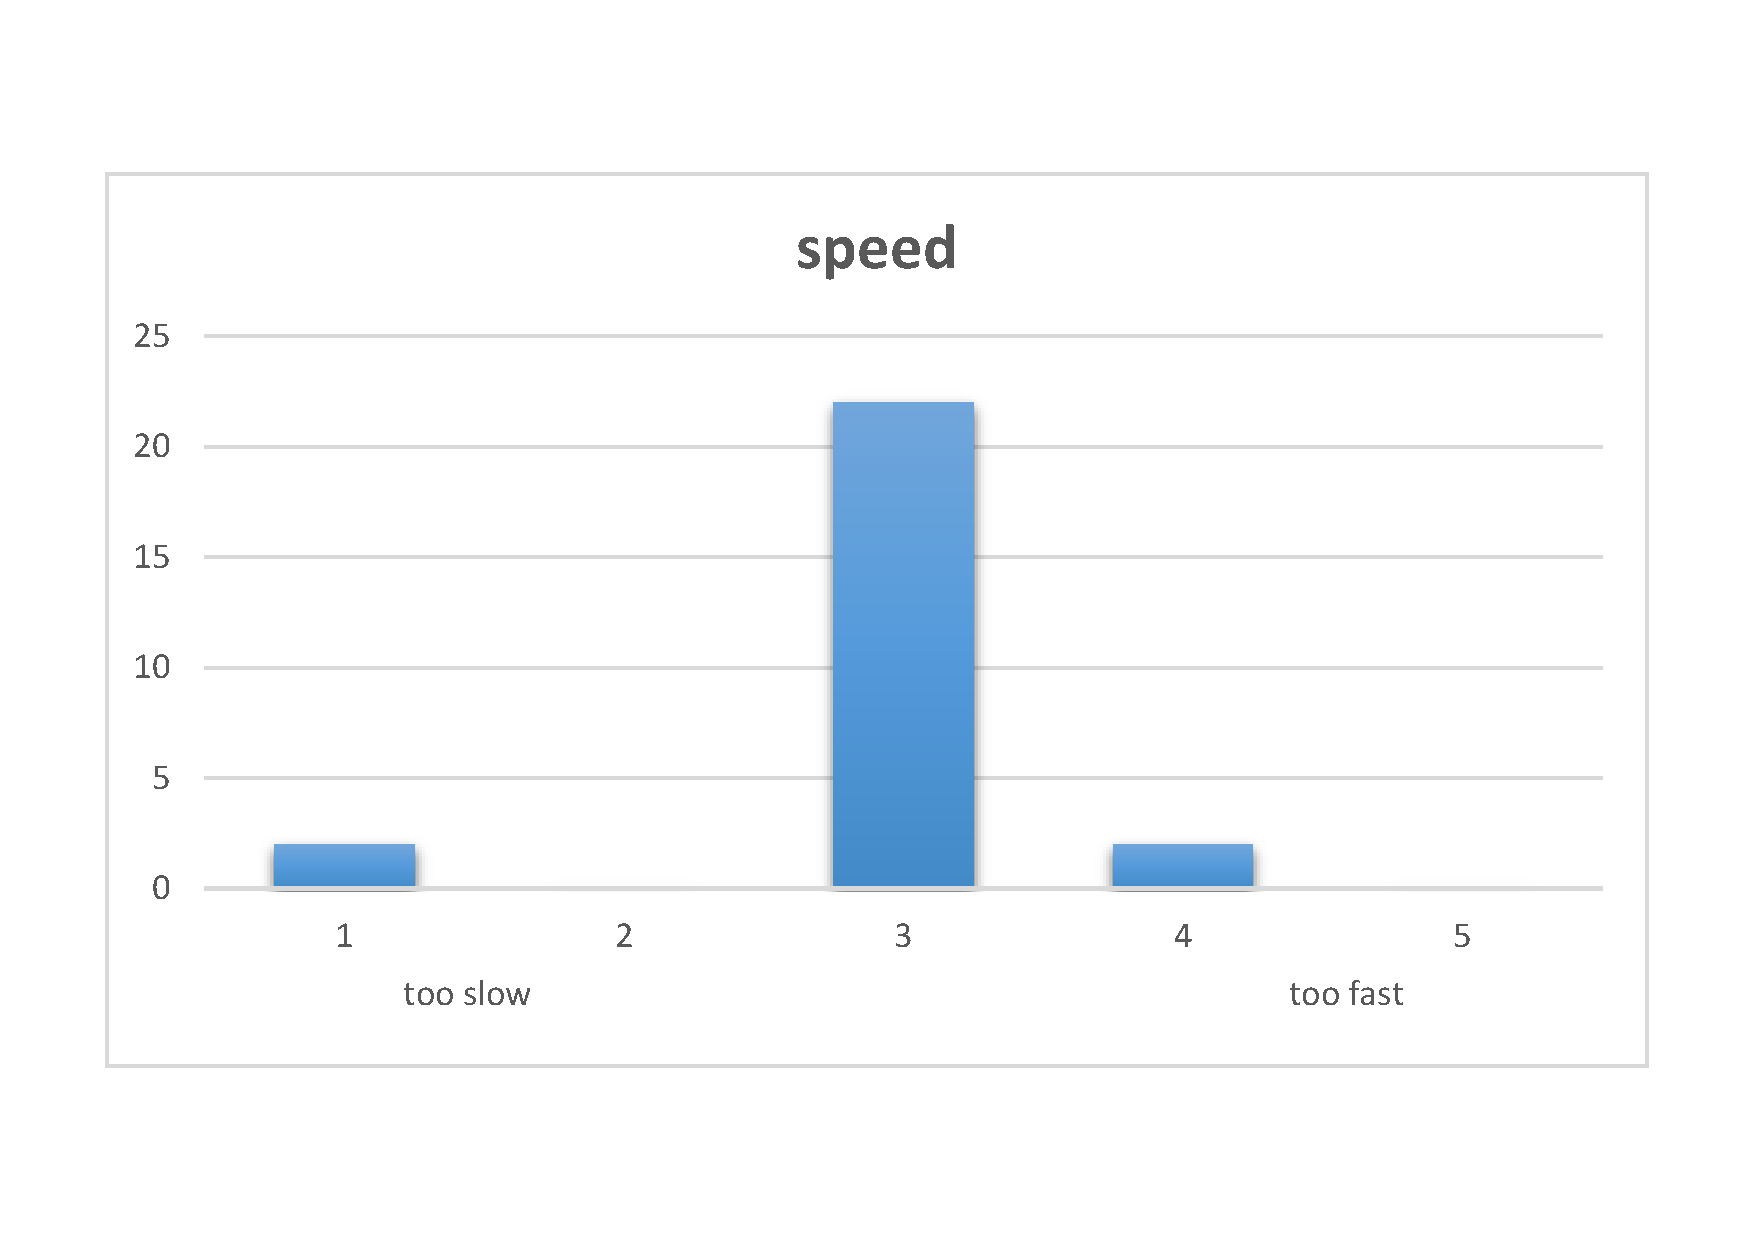
\includegraphics[width=0.49\textwidth]{speed.pdf}}
\hfill\null % 
\end{figure} 

\end{document}
